L'application se lance lors d'un double clique sur l'exécutable.

\section{Se connecter}
La première fen\^etre à apparaitre est l'interface de connexion ci-dessous :
\begin{figure}[!h]
\centering
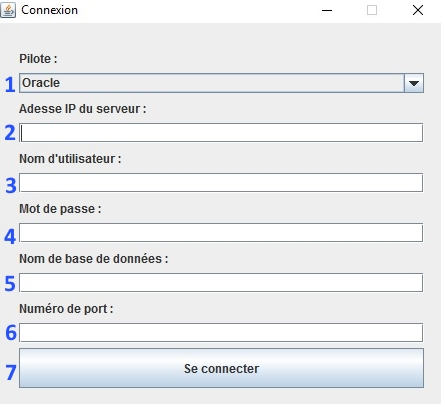
\includegraphics[width=10cm]{./images/manuel/se_connecter.jpg}
\caption{IHM - Se connecter}
\label{se_connecter}
\end{figure}

Afin de se connecter il faut renseigner les différents champs présents dans la fen\^etre.

\begin{enumerate}
\item choix du SGBD* (Oracle, MySQL).
\item Adresse IP du serveur ou est stockée votre base de données.
\item Nom d'utilisateur utilisé pour vous connecter à votre base de données. 
\item Mot de passe utilisé pour vous connecter à votre base de données.
\item Nom de la base de données.
\item Numéros de port du serveur ou est stockée votre base de données.
\item Cliquer sur le bouton \textbf{se connecter} pour tenter de se connecter au serveur.
\end{enumerate}

Connexion aux serveurs de l'IUT si vous \^etes étudiant :\\

\textbf{Oracle}
\begin{itemize}
\item SGBD : Oracle
\item Adresse IP : 162.38.222.149
\item Nom d'utilisateur : <nom-de-famille><première-lettre-du-prenom>
\item Mot de passe : <votre-INE>
\item Nom de la base de données : IUT
\item Numéros de port : 1521 \\
\end{itemize}

\textbf{MySQL}
\begin{itemize}
\item SGBD : MySQL
\item Adresse IP : 162.38.222.142
\item Nom d'utilisateur : <nom-de-famille><première-lettre-du-prenom>
\item Mot de passe : <votre-INE>
\item Nom de la base de données : <nom-de-famille><première-lettre-du-prenom>
\item Numéros de port : 3306
\end{itemize}

\section{Créer une table}
Dans le menu principal de l'application, cliquez sur le bouton \textbf{LDD : créer tables} pour ouvrir la fen\^etre de création de tables.

\begin{figure}[!h]
\centering
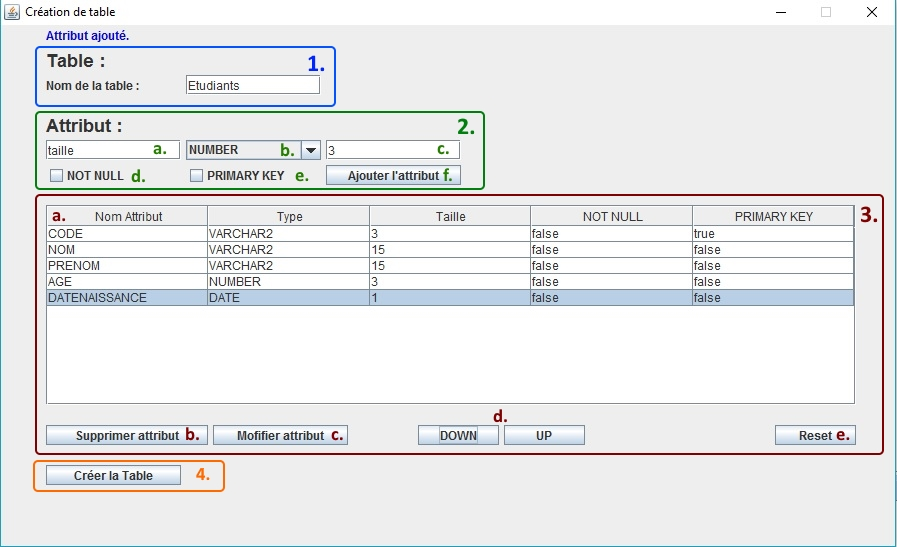
\includegraphics[width=14cm]{./images/manuel/creer_table.jpg}
\caption{IHM - Créer table}
\label{creer_table}
\end{figure}

\begin{enumerate}
\item Nom de ta table - \textit{ex : Etudiants}

\item Gestion des caractéristiques d'un attribut :
\begin{enumerate}
\item Nom - \textit{ex : codeEtudiant}
\item Type - \textit{ex : VARCHAR2}
\item Taille - \textit{ex : 15}
\item A cocher pour que l'attribut ne soit jamais null.
\item A cocher pour que l'attribut soit une clé primaire de votre table.
\item Cliquer sur le bouton \textbf{Ajouter l'attribut} pour tenter d'ajouter un attribut à la table.
\end{enumerate}

\item Gestion des attributs ajoutés :
\begin{enumerate}
\item Tableau contenant les attributs ajoutés avec le bouton <Ajouter l'attribut>.
\item Cliquer sur le bouton \textbf{Supprimer l'attribut} pour supprimer l'attribut sélectionné dans le tableau.
\item Cliquer sur le bouton \textbf{Modifier l'attribut} pour modifier l'attribut sélectionné dans le tableau. 
Les caractéristiques de l'attribut sélectionné sont à modifier dans la zone de gestion des caractéristiques d'un attribut. 
Vous pouvez ensuite valider ou annuler votre modification.
\item Cliquer sur les boutons \textbf{UP/DOWN} pour modifier l'odre des attributs dans le tableau. 
\item Cliquer sur le bouton \textbf{Reset} pour remettre à zéro la fen\^etre de création.
\end{enumerate}

\item Cliquer sur le bouton \textbf{Créer la table} pour tenter la création de la table.
\end{enumerate}





\section{Modifier une table}
Dans le menu principal de l'application, clique sur le bouton \textbf{LDD : modifier tables} pour ouvrir la fenêtre de modification de tables.


\begin{figure}[!h]
\centering
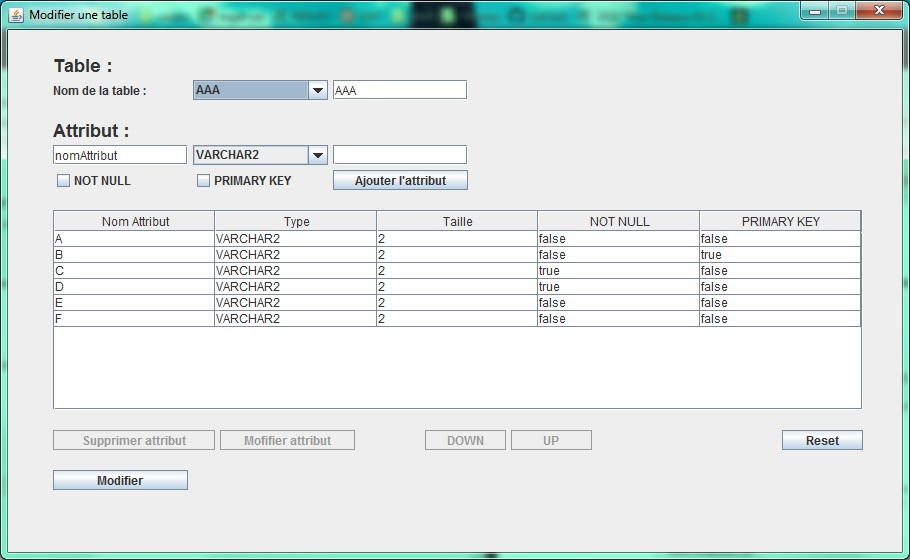
\includegraphics[width=10cm]{./images/manuel/modifier_tables.jpg}
\caption{IHM - Modifier une table}
\label{modifier_table}
\end{figure}

Cette fenêtre est identique à la fenêtre de Création d'une table, à la différence qu'il est possible de sélectionner une table déjà existante dans la \bdd. 

Il est possible de modifier une table existante avec le bouton \textbf{modifier}, sans perdre de données mais il est possible que certaines soient perdus lors de la modification :
\begin{itemize}
\item suppression d'un attribut clé étrangère couplé avec un second attribut
\item modification du type de l'attribut pouvant altérer les données.
\end{itemize}





\section{Supprimer une table}
Dans le menu principal de l'application, cliquer sur le bouton \textbf{LDD : supprimer tables} pour ouvrir la fen\^etre de suppression de tables.

\begin{figure}[!h]
\centering
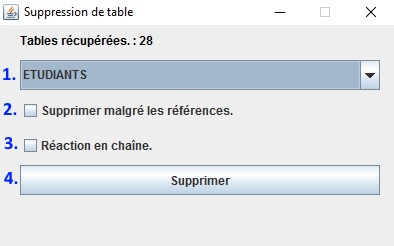
\includegraphics[width=8cm]{./images/manuel/supprimer_table.jpg}
\caption{IHM - Supprimer une table}
\label{supprimer_table}
\end{figure}

\begin{enumerate}
\item Choisir la table à supprimer.
\item A cocher pour supprimer sans prendre en compte les références des autres tables sur celle à supprimer.
\item A cocher pour supprimer la table sélectionnée puis toutes celles qui font référence à cette table et ceci récursivement.
\item Cliquer sur le bouton \textbf{Supprimer} pour tenter la suppression de la table.
\end{enumerate}

\section{Requ\^etes SQL}
Dans le menu principal de l'application, cliquer sur le bouton \textbf{SQL} pour ouvrir la fen\^etre du mode requ\^etes SQL.
\begin{figure}[!h]
\centering
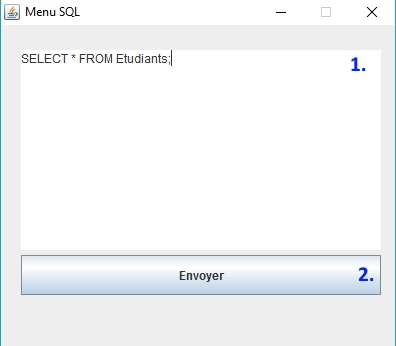
\includegraphics[width=6cm]{./images/manuel/sql.jpg}
\caption{IHM - SQL}
\label{sql}
\end{figure}

\begin{enumerate}
\item Ecrire la requ\^ete dans la zone de saisie - \textit{ex : SELECT * FROM Etudiants;} 
\item Cliquer sur le bouton \textbf{Envoyer} pour tenter d'exécuter la requ\^ete.
Une fenêtre s'ouvre indiquant le résultat de la requ\^ete si la syntaxe est correcte.
\end{enumerate}

\begin{figure}[!h]
\centering
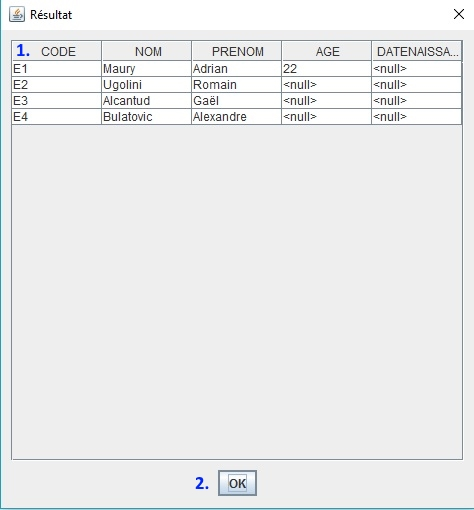
\includegraphics[width=8cm]{./images/manuel/sql_result.jpg}
\caption{IHM - Résultat SQL}
\label{sql_result}
\end{figure}

\begin{enumerate}
\item Résultat de la requ\^ete.
\item Cliquer sur le bouton \textbf{OK} pour fermer la fen\^tre de résultat.
\end{enumerate}

\section{CRUD* les tuples des tables}
Dans le menu principal de l'application, cliquer sur le bouton \textbf{CRUD} pour ouvrir la fen\^etre de gestion des tuples des tables.
\begin{figure}[!h]
\centering
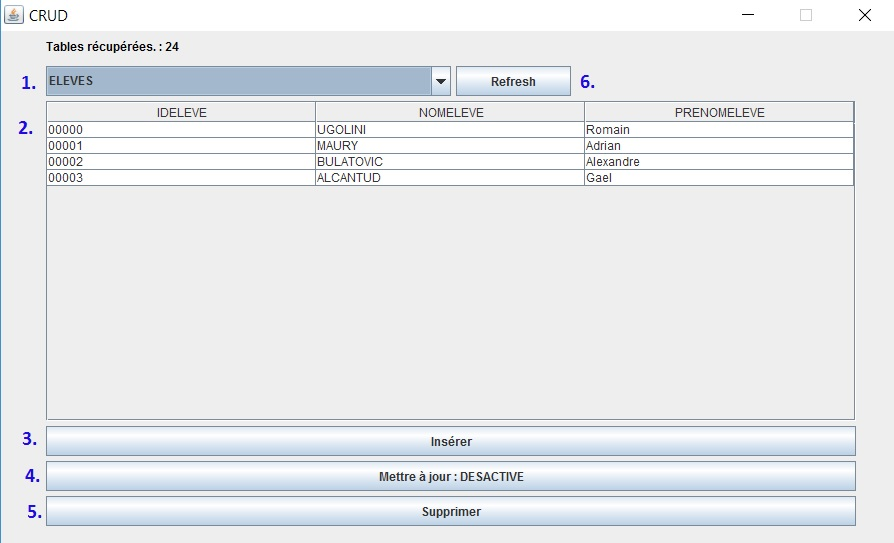
\includegraphics[width=12cm]{./images/manuel/crud.jpg}
\caption{IHM - CRUD}
\label{crud}
\end{figure}

\begin{enumerate}
\item Choisir la table.
\item Tableau contenant les différents tuples de la table sélectionnée.
\item Cliquer sur le bouton \textbf{Insérer} pour ajouter un tuple à la table. Il faut ensuite remplir les informations du nouveau tuple
dans la ligne vide qui s'est ajouté au tableau.
\item Cliquer sur le bouton \textbf{Mettre à jour} pour modifier un tuple de la table. Il faut ensuite modifer les informations du tableau et 
appuyer sur la touche entrée à chaque modification. Quitter le mode modification en cliquant une nouvelle fois sur le bouton \textbf{Mettre à jour}.
\item Cliquer sur le bouton \textbf{Supprimer} pour supprimer le tuple selectionné.
\end{enumerate}

\section{Ajouter et Supprimer des contraintes}
